\documentclass[12pt]{article}
\usepackage[utf8]{inputenc}
\pagenumbering{arabic}
\usepackage{graphicx}
\usepackage{amstext}
\usepackage[usenames, dvipsnames]{color}
\usepackage{array}
\usepackage{float}
\usepackage{enumitem}
\usepackage[top=1.5in]{geometry}
\usepackage{subcaption}
\graphicspath{{images/}}
\usepackage[]{algorithm2e}
\usepackage{amsmath}

\begin{document}

\begin{titlepage}
    \begin{center}
    \begin{figure}
        \centering
        
\includegraphics[scale=0.2]{logoPolimi.png}
        \vspace{1.5cm}
    \end{figure}

    \Huge\textbf{Software Engineering 2 Project - TrackMe}
    \rule{12cm}{0.5pt}
    \Huge\textbf{Design Document - V1.0}
    \vspace{1mm}
    \newline
    \today
    \end{center}
    
    \vspace{3cm}
    
    \begin{flushleft}
        \LARGE\textbf{Authors: }
        \newline\newline
        \Large\texttt{}{Michiel Janssen \\ Erbol Kasenov \\ Lorenzo Casalini}
    \end{flushleft}
\end{titlepage}

\newpage
  \tableofcontents
\newpage
\section{Introduction}

\subsection{Purpose}
The main purpose of the Software Design Document (or just Design Document) is to provide a more technical and detailed description than the RASD about the TrackMe application system. This document describes how TrackMe is designed and planned, identifying its main components and the interfaces between them. It also guides the software development team and other interested parties through the architecture of the software project, stating what has to be implemented and how to do it.
\vspace{3mm}
\newline 
More precisely, the document presents:
\begin{itemize}
    \item Overview of the high level architecture
    \item The main components and their interfaces provided one for another
    \item The r untime behavior
    \item The design patterns
    \item The algorithm design of the most critical parts of the application
    \item Implementation plan
    \item Integration plan
    \item Testing plan
\end{itemize}
The purpose of this document is to provide an overall guidance to the architecture of the software product.



\subsection{Scope}
TrackMe is a company that wants to develop a software-based service allowing third parties to monitor the location and health status of individuals. The main service, Data4Help, supports the registration of individuals (of any age) and third parties. Upon registration the individual agrees that TrackMe acquires their data. This data can be obtained from smartwatches or similar devices. After registration a third party can request the following things:
\begin{itemize}
\item Access the data of a specific individual by entering a unique number or code. TrackMe passes the request to the specific individual who can accept or refuse the data acquisition.
\item Access anonymized data of groups of individuals given by a specific constraint e.g.: every individual older than 30 years, every individual that is male or female, etc. These requests are handled and approved by TrackMe if and only if TrackMe can guarantee that they are able to properly anonymize the requested data.
\end{itemize}
As soon as a data request is approved, TrackMe makes the previously saved data available to the third party. The service also allows a third party to subscribe to new data and listen to new data as soon as they are produced. With the data acquired through Data4Help, it will be also possible to offer two other services based on the retrieved data. The first service is a personalized and non-intrusive SOS service, called AutomatedSOS, to help elderly people. This service monitors the health status of subscribed customers and sends an ambulance to this specific customer if some parameters are below a certain threshold. The reaction time should be less than 5 seconds from the time the parameters are below the certain threshold.
The second service, called Track4Run, allows organizers to define a path for a run, participants to enroll to a certain run and spectators to see the position of all current running participants on a map.


\subsection{Definitions, Acronyms, Abbreviations}

\subsubsection{Definitions}

\begin{itemize}
\item \textit{Visitor}: A person who uses TrackMe for the first time, and is not yet registered. This can be an individual or a third party. After a successful registration process the person becomes an individual and is now able to use TrackMe services.
\item \textit{Individual}: A registered person who uses TrackMe for monitoring his location and health status.
\item \textit{Third-parties}: A registered organization that wants to access the location and health status of specific individual by giving a social security number of that individual.
\item \textit{System}: defines the overall set of software components that implement the required functionality.
\end{itemize}
\newpage 
\subsubsection{Acronyms}

\begin{itemize}
    \item \textit{API}: Application Programming Interfaces
    \item \textit{RASD:} Requirements Analysis and Specifications Document
    \item \textit{DD}: Design Document
    \item \textit{DB}: Database
    \item \textit{DBMS}: Database Management System
    \item \textit{ER}: Entity Relationship Model
    \item \textit{SQL}: Structured Query Language
    \item \textit{UX Diagram}: User Experience Diagram
    \item \textit{JSON:} JavaScript Object Notation
    \item \textit{REST:} Representational State Transfer
    \item \textit{EJB:} Enterprise JavaBeans
    \item \textit{JEE:} Java Platform, Enterprise Edition

\end{itemize}

\subsubsection{Abbreviations}
\textit{Gn}: Goal defined with index n.\newline
\textit{Rn}: Functional Requirement defined with index n.
\subsection{Revision History}
\textbf{Version 1.0:} Initial Release

\subsection{Reference Documents}
\begin{itemize}
    \item RASD V1.0 produced before
    \item Assignment document: Mandatory Project Assignment AY 2018-2019.pdf
    \item Design Patterns by Jason McDonald (dzone.com/refcardz/design-patterns)
\end{itemize}

\newpage
\subsection{Document Structure}
Other than this introductory chapter, this DD is organized in seven more chapters.
Chapter two is meant to \textbf{provide different types of views over the system:}
\begin{itemize}
     \item High level components and their interaction : this sections gives a global view of the components
     of the application and how they communicate
     \item Component view : this sections gives a more detailed view of the
     components of the applications

    \item  Deploying view : this section shows the components that must be
    deployed to have the application running correctly.

    \item  Runtime view : sequence diagrams are represented in this section to
    show the course of the different tasks of our application
    \item Component interfaces : the interfaces between the components are
    presented in this section

    \item Selected architectural styles and patterns : this section explain the
    architectural choices taken during the creation of the application


    \item Other design decisions
\end{itemize}

\noindent 
In the third chapter the most \textbf{relevant algorithms} are analyzed and discussed with the appropriate
detail and depth, in order to describe the way the system’s most critical operations are driven and executed
. Pseudo code is used for the algorithms in order to hide unnecessary implementation details.
The fourth chapter deals with the \textbf{user interface design}. This chapter mainly refers to the mockups 
provided in the RASD, but it will also include some details on the user interaction with the UI, illustrated
by a UX Diagram.
The fifth chapter explains how the \textbf{requirements defined in the RASD are fulfilled by the design 
decisions} that were taken, and how these \textbf{requirements map} to the design elements and decisions 
defined in the DD.
In the sixth chapter, a \textbf{implementation, integration and test plan} is provided, defining the 
order in which the different subcomponents of the system will be implemented, the 
order in which they will be integrated and how this integration will be tested alongside with the
development of the system.
In the seventh chapter the \textbf{effort spent by each of the group members} is described by specifying the
number of hours each member of the group worked on the development of this document and, on the final
chapter, \textbf{the tools we used to develop this DD are specified.}  


\section{Architectural design}

\subsection{Overview: High-level components and their interaction}
In the following paragraphs a general overview of how the system is architected will be presented,
especially focused on the different logically separated layers. As described on the RASD, TrackMe is
supposed to be fully scalable and portable, so a layered architecture is the one that best fits these
requirements. Given that the system only provides an Application interface, there’s no need for a fourth
layer isolating the web server from the application server.
With this in mind, the system will have a three-layer architecture, organized as shown below:

\begin{figure}[H]
\centering
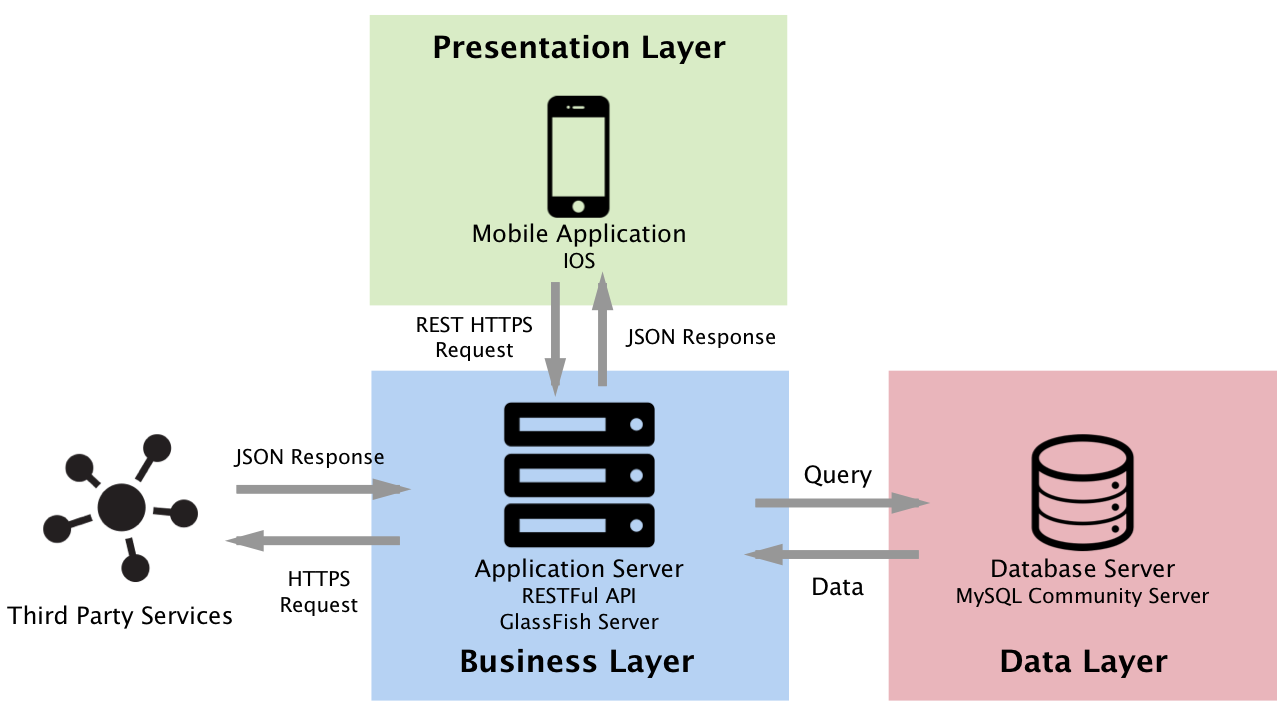
\includegraphics[scale=0.6]{highLevelView.png}
\label{fig:highLevelView}
\caption{High Level View of the system's architecture.}
\end{figure}
\noindent 
\begin{itemize}
    \item \textbf{Presentation Layer:} is the most external layer of the system, and is respon- sible for handling all GUI communication and logic. This layer does not handle data or process business rules, but it forwards all the requests to the layers bellow and translates the system operations results of these requests to something that users can understand. It is the only layer of the system that users can access directly and interact with.
    \newpage
    \item \textbf{Business Layer:} implements all core functionality of the system. It's in this layer that the application logic and business rules are implemented, in particular, all the operations related to a individual or third party account and health data creation are performed by components of this layer. This layer interacts with the APIs exposed by the Data Layer in order to store and retrieve data. The business layer also depends on some third party systems and the external services they provide (specifically for the implementation of the health data creation we rely on external devices to monitor data). These external services are directly invoked by some of the classes of the Business Layer using a public API provided by those.
    \item \textbf{Data Layer:} is the lowest layer of the architecture and includes the data persistence mechanisms responsible for data storage and management. It also provides an API to the Business Layer that exposes methods of managing the stored data without creating dependencies on the data storage mechanisms, promoting the encapsulation of the persistence mechanisms and avoiding data exposition.
    \item \textbf{Third Parties:} Even though they don't belong to any particular layer, these services are illustrated in the figure above in order to highlight that the interaction with the hird parties will happen at the level of the Business Layer.
\end{itemize}

\subsection{Component view}
The main function of this section is to present a more detailed description of the components that must be
developed as part of TrackMe. In the following diagram, we can see the component view of the system (the
more complex components will be analyzed in further detail).

\begin{figure}[H]
\centering
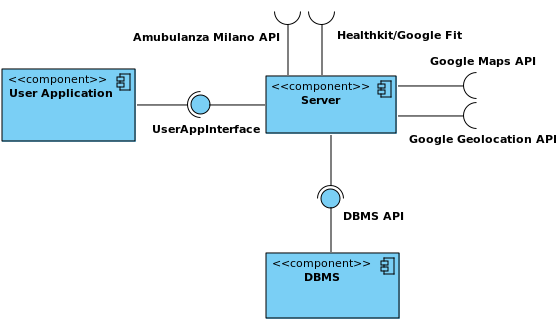
\includegraphics[scale=0.5]{ComponentDiagram1.png}
\label{fig:ComponentDiagram1}
\caption{Component Diagram of the system.}
\end{figure}
\newpage
\noindent 
The \textbf{User Application} is the component responsible for providing the user interfaces that allow
the user to interact with the system and all of its functionality. Since a thin-client architecture is being
used to implement a client/server architecture, the bulk of the data processing occurs on the server.
Given this, the User Application component will act as a simple "terminal" to send requests to the server,
being therefore quite simple and not needed to go into further detail.
\newline \noindent The \textbf{Server} is the main component of the system, responsible for the data
processing in order to provide all of the system’s functionality. Given its complexity, it will be analyzed
in further detail later in this section.
\newline \noindent The \textbf{DBMS} is the component responsible for storing and retrieving data in a 
persistent and reliable way. Instead of implementing this component from scratch, a commercial solution 
shall be used (MySQL for example).

\subsubsection{Server detailed analysis}

\vspace{3mm}
\noindent Being the most complex component of the system, it is useful to analyze in detail the Server's 
constitution. As mentioned previously, this component is primarily responsible for all operations related 
to the system's functionality. More specifically, this component is divided into six sub-components, each 
related to a different kind of functionality and operations (diagram can be found in figure ~\ref{fig:serverComponentView}):

\begin{itemize}
    \item The \textbf{Router} sub-component receives the requests from the User Application and forwards (routes) them to the corresponding controller.
    \item The \textbf{Health Data Controller} sub-component is the one who performs all the necessary
          operations that allow the user to collect all his health data acquired and made through external devices. This module is the one with more external interfaces since it needs to gather all health data from individuals in combination with the location from the external devices. This sub-component is also responsible to communicate with the Ambulanza Milano API, so when a certain parameter is below a certain value the system can immediately ask to send the closest ambulance to the individual in danger. 
    \item The \textbf{Account Controller} sub-component implements all the methods for inserting or updating information about the users. More specifically, it allows the creation of new users (registration of visitors) and login of already existing users.
    \item The \textbf{Run Controller} sub-component implements all the methods so that every user can organize a path for a run and every individual can participate in a run or spectate runners. It uses information from the Health Data Controller and Account Controller to fulfill this requirements.

    \item The \textbf{Data Access Controller} sub-component (and all of its sub-components) manages the behavior and data of the application domain and responds to requests or instructions by the respective controller.
    \item The \textbf{Data Mappers} sub-component is a layer of software which separates the model from the database and acts as a "middle-man", the backend, for the interactions between these two.
\end{itemize}
\subsubsection{Database detailed analysis}
The following ER provides a graphical representation of the conceptual model of the database.
\vspace{20mm}

\begin{figure}[H]
\centering
\centerline{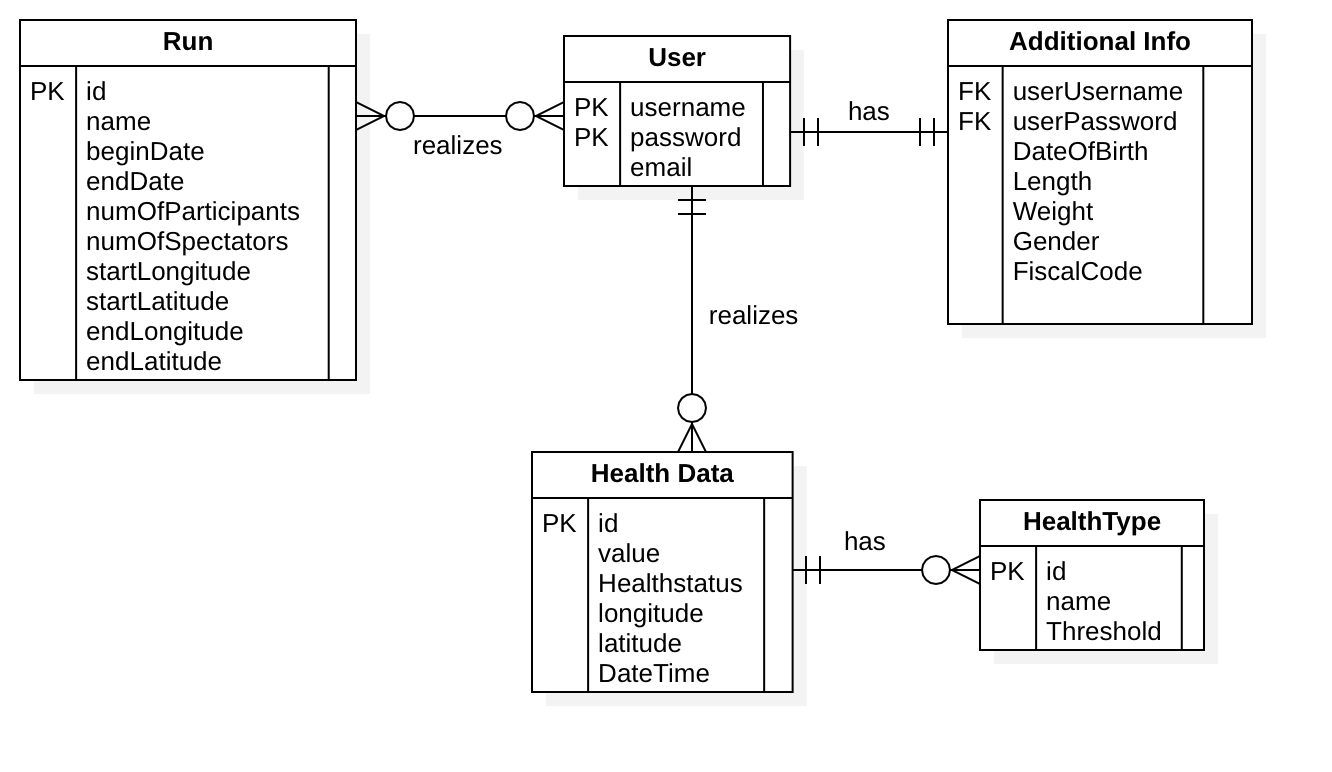
\includegraphics[scale=0.4]{databaseTrackMe.png}}
\caption{Database ER.}
\label{fig:databaseTrackMe}
\end{figure}



\begin{figure}[H]
\centering
\centerline{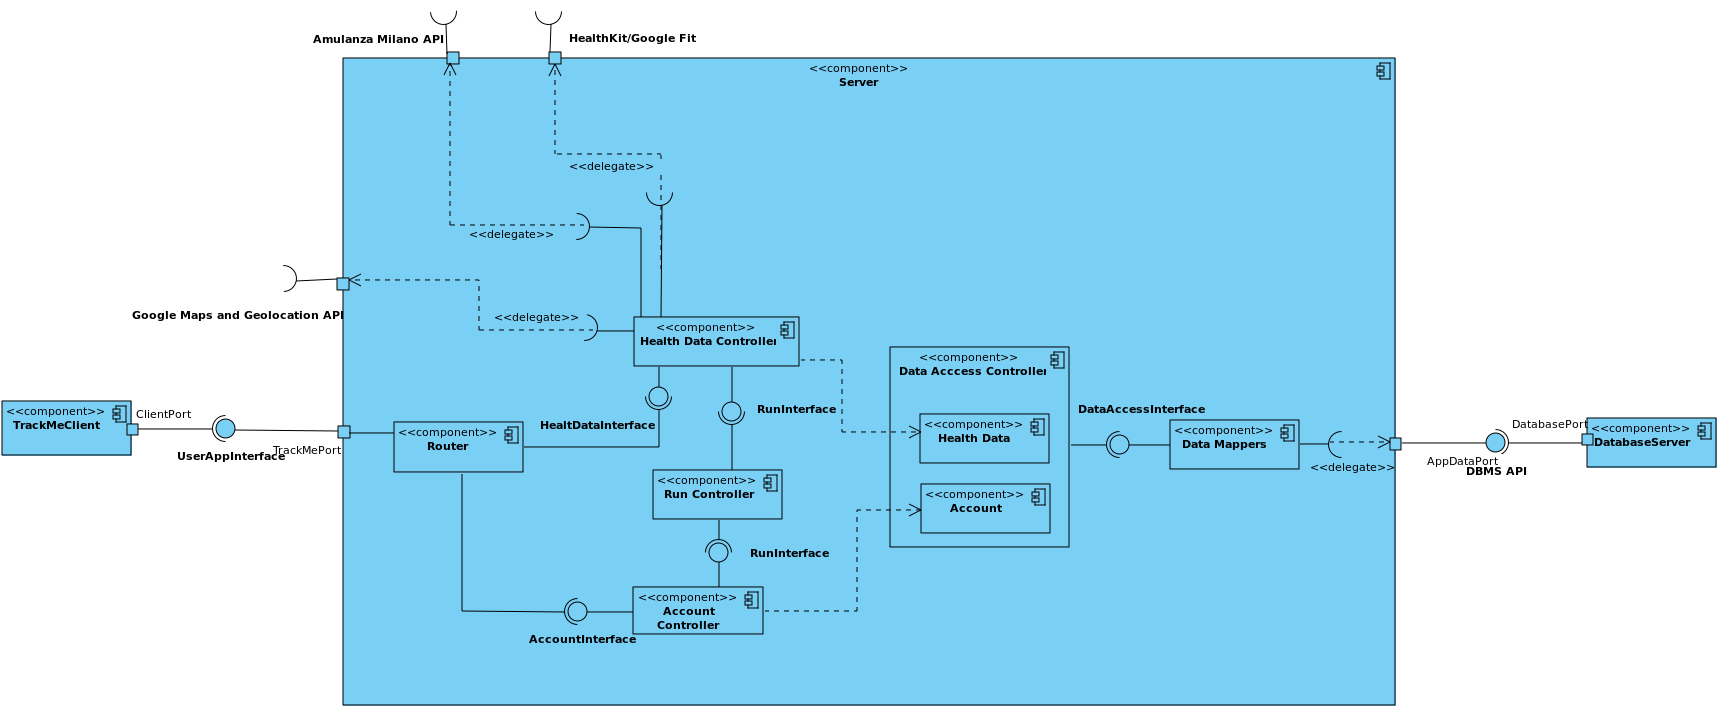
\includegraphics[scale=0.33, angle=-90,origin=c]{serverComponentView.png}}
\caption{View of Server Component in detail.}
\label{fig:serverComponentView}
\end{figure}


\subsection{Deployment view}
The main purpose of this section is to show how the software components described above are going to be 
deployed in the system's hardware infrastructures. This characteristic makes the developer's task easier 
since the mapping between software and hardware becomes explicit. The deployment diagram in figure ~\ref{fig:DeploymentView} shows the architecture of the system as deployment (distribution) of software artifacts
to deployment targets. TrackMe requires deployment of software on the following nodes:
\begin{enumerate}
    \item \textbf{User Application:} this is the application (TrackMe) that will be used by the user. The user will be able to get information from the main TrackMe server.
    \item \textbf{TrackMe server:} the main logic of the application will be deployed here. This server will communicate with all the other nodes. It will gather information from the external services (API's), manage user accounts and saved health data from the Database server and take requests and send back responses to the user.
    \item \textbf{Database server:} it will store all the persistent data for the users such as usernames and passwords, as well as their health data and data about the organization of runs.
    \item \textbf{External server:} it will only provide services to enrich the application. For example, Google Maps/Geolocation is used to locate an individual, HealthKit/Google Fit is used to track the health of an individual, etc.
     
\end{enumerate}


\begin{figure}[H]
\centering
\centerline{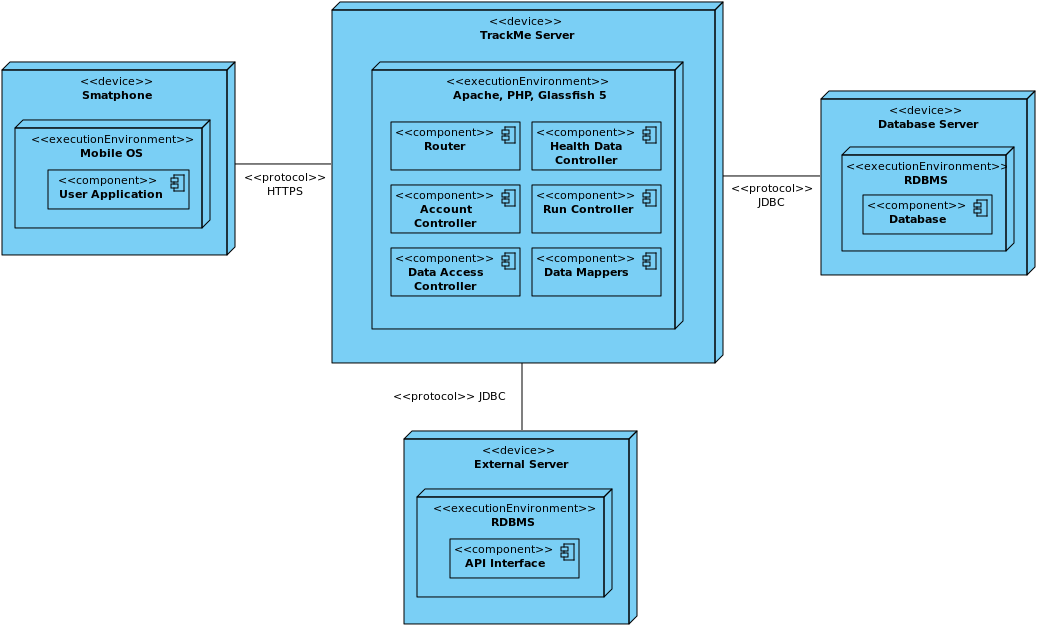
\includegraphics[scale=0.45]{DeploymentView.png}}
\caption{Deployment View of the system.}
\label{fig:DeploymentView}
\end{figure}

\subsection{Runtime view}
The following diagrams are intended to describe the interactions between the main system components when 
performing a sample amount of functionality. These diagrams are still a high-level view of the system, 
since the function names or even the functions themselves may change during the development process.

\begin{itemize}
    \item \textbf{Section 2.4.1:} in this sequence, the process of logging in a user is shown. The user fills in his credentials and passes it to the user application which checks if the provided data is valid. The router forwards the validity request to the DBMS to check if a match for the given username and password is found in the DB. If and only if the filled in data is valid (correct credentials) the user application displays a success. The result of this success is that the user is now successfully logged in and can use the TrackMe application. If no success has occurred the user application displays an error.
    \newpage 
    \item \textbf{Section 2.4.2:} in this sequence, the process of creating new health data for a user is shown. The component mainly used for this operation is the Health Data Controller. It's the user application (and not the user himself) who creates this health data. The user is not the one who is responsible for making the health data, he doesn't need to push on a button to retrieve new health data. The first time a user uses TrackMe, the user gives permission to TrackMe to track his health and further retrieving of available data is done automatically in the background by the user application. First the Health Data Controller retrieves specific data from HealthKit or Google Fit by entering the HealthDataDetails (this is usually a username). After retrieving the health data from the user, the Health Data Controller internally checks the healthstatus of the user. If and only if the threshold of a certain parameter, defined for each type health data, is violated (person is in danger) the system communicates with the Ambulanza Milano API and they will send an ambulance to the person in question. After that we try to make the health data. Only is the health data is makeable (health data won't be makeable if e.g.: you want to monitor the blood pressure of a user but this user isn't using a external device to measure the blood pressure. Therefore we can't retrieve this data and it's not makeable) it willed be placed inside the Health Data Controller health data queue. This queue is then uploaded to the database to store health data for each user. If nothing goes wrong we have successfully made new health data, otherwise an error will occur in the background stating that something went wrong when uploading data to the database. Last but not least if health data is not makeable there will also occur an error in the background of the user application.
    \item \textbf{Section 2.4.3:} in this sequence, the process of requesting health data of a single individual is shown. First a third party decides that it wants to monitor the health data of a specific individual by giving in the HealthDataDetails (usually a fiscal code of the individual). The router forwards this request to the Health Data Controller who in turn forwards the request to the Account Controller. The Account Controller is responsible for forwarding the request to the individual in question. This individual receives a pop-up notification where it can decide to accept or decline the health data request. If the individual approves the request, the Health Data Controller can retrieve the previously saved health data from the database and forward it to the requesting third party. This also allows the third party to subscribe to new data and receive them as soon as they are produced. If the individual declines the request an error notification occurs on the third party user application side.
    \newpage
    \item \textbf{Section 2.4.4:} in this sequence, the process of requesting anonymized health data of a group of individuals is shown. First a third party decides that it wants to monitor the anonymized health data of group individuals by giving in the HealthDataDetails (for instance, all those individuals living in a certain geographical area, all those individuals of a specific age range, etc.). The router forwards this request to the Health Data Controller. The Health Data Controller is responsible for evaluating/handling the request. We assume that TrackMe, more specific the Health Data Controller, will accept any request for which the number of individuals whose data satisfy the request is higher than 1000. If the data can be anonymized, the Health Data Controller can retrieve the previously saved health data from the database and forward it to the requesting third party. This also allows the third party to subscribe to new data and receive them as soon as they are produced. If the data can't be anonymized an error notification occurs on the third party user application side.

    
    \item \textbf{Section 2.4.5:} in this sequence, the process of creating new run for a user is shown. The component mainly used for this operation is the Run Controller. First the user chooses to organize a run and this request is bypassed to the Run Controller. The Run Controller first creates a path for a run defined by the user who organizes it (assuming that in the meantime users already subscribed to participate or spectate the run). Then we retrieve all participating users and spectators by communicating with the database. For participating users we retrieve user information as well as health data (to monitor them while running) and for spectators we only retrieve user information to know who is spectating the run. A run is makeable if and only if the run has a reasonable path. If the run is makeable we try to upload and store the most important information concerning the run to the database. If this succeeds we display a success, otherwise an error. The same error occurs when a run is not makeable.
\end{itemize}

\subsubsection{User Login}

\begin{figure}[H]
    \centering
    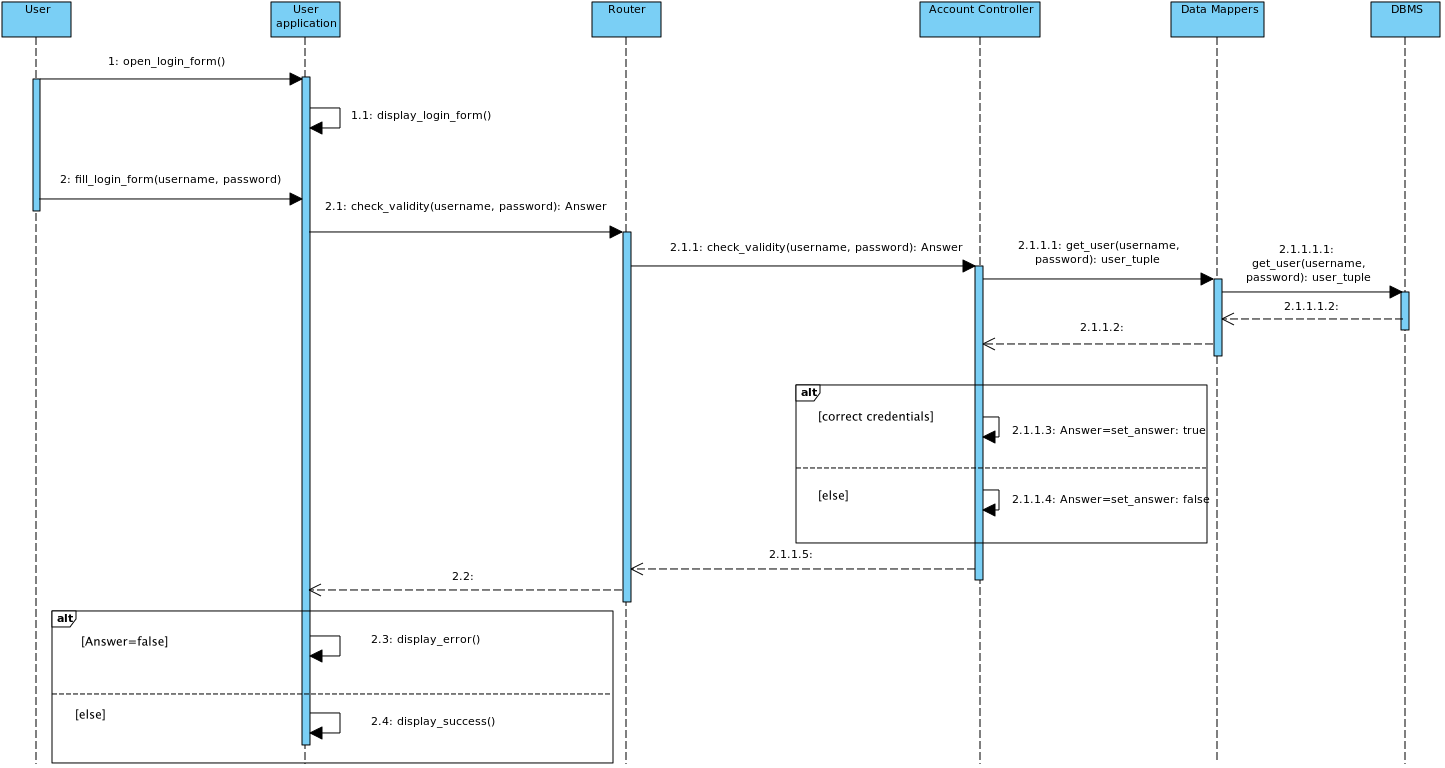
\includegraphics[scale=0.37, angle=-90, origin=c]{loginRuntimeView.png}
    \caption{User Login.}
    \label{fig:loginRuntimeView}
\end{figure}

\subsubsection{Create Health Data}

\begin{figure}[H]
    \centering
    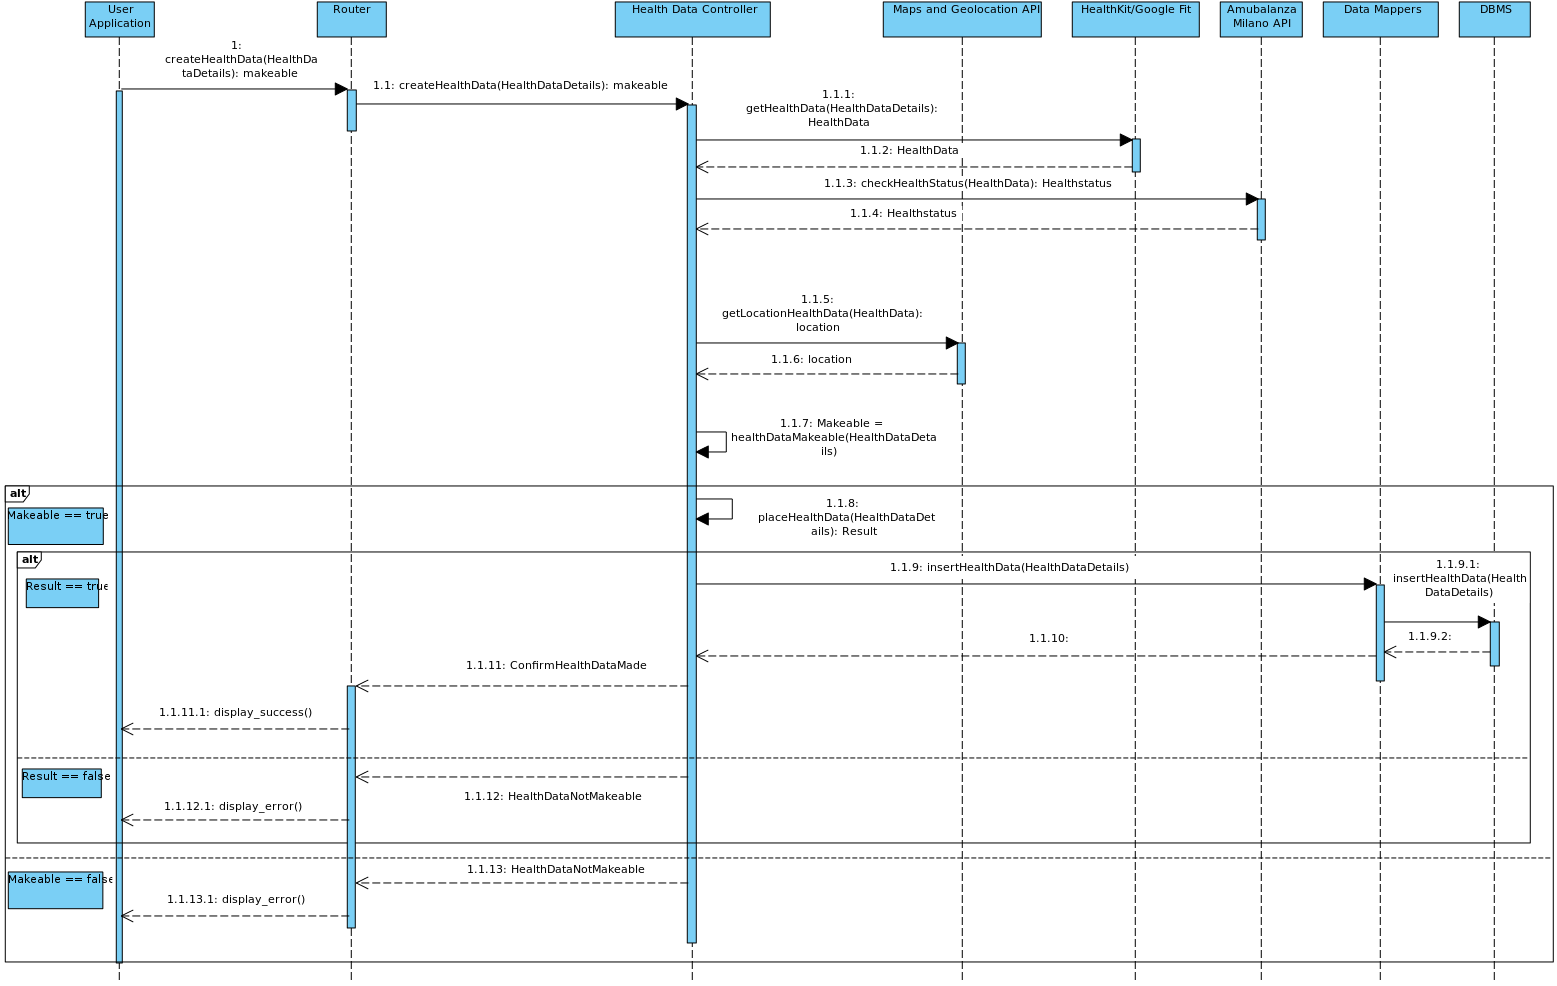
\includegraphics[scale=0.35, angle=-90, origin=c]{createHealthData.png}
    \caption{Health Data created for User.}
    \label{fig:createHealthData}
\end{figure}

\subsubsection{Request Health Data single individual}

\begin{figure}[H]
    \centering
    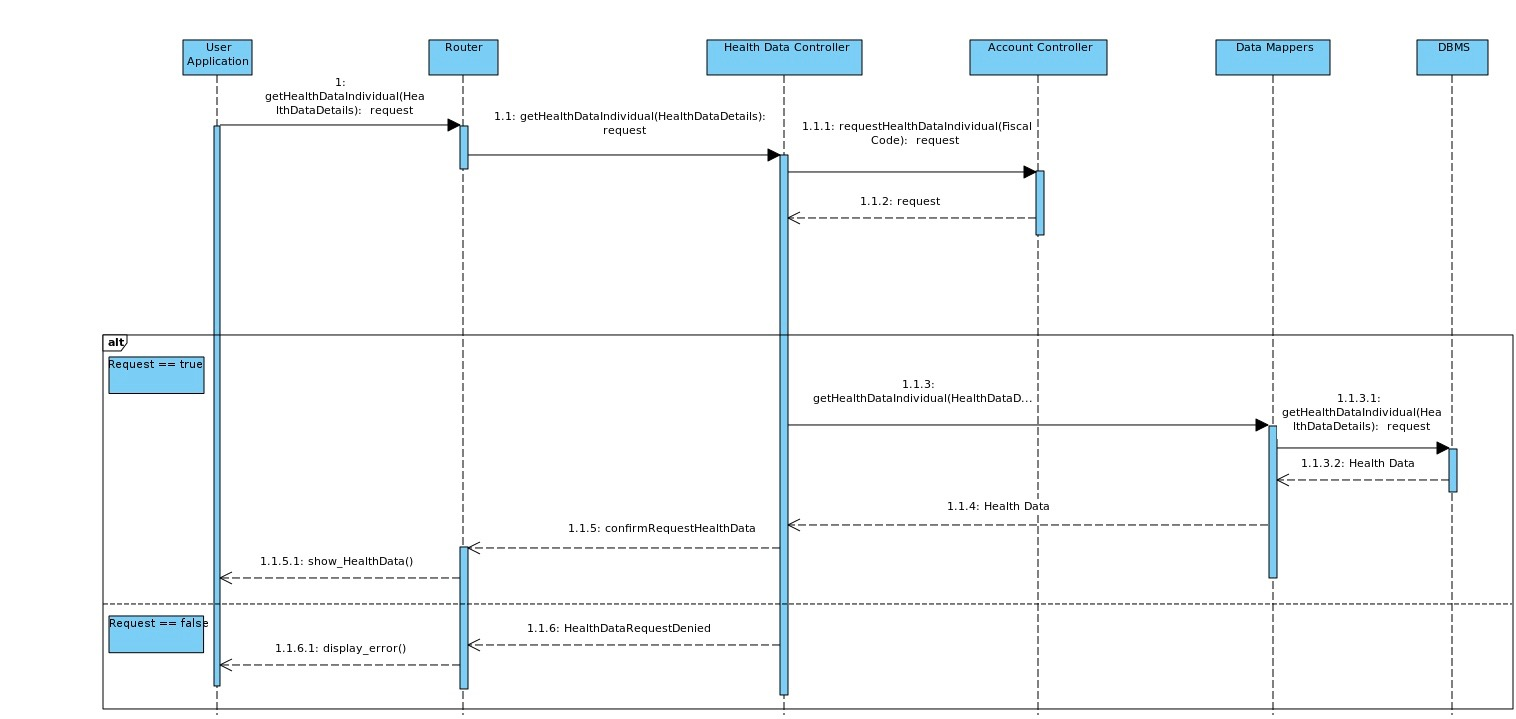
\includegraphics[scale=0.35, angle=-90, origin=c]{getHealthDataIndividual.jpeg}
    \caption{Request for the Health Data of a single individual.}
    \label{fig:getHealthDataIndividual}
\end{figure}

\subsubsection{Request Health Data anonymized group}

\begin{figure}[H]
    \centering
    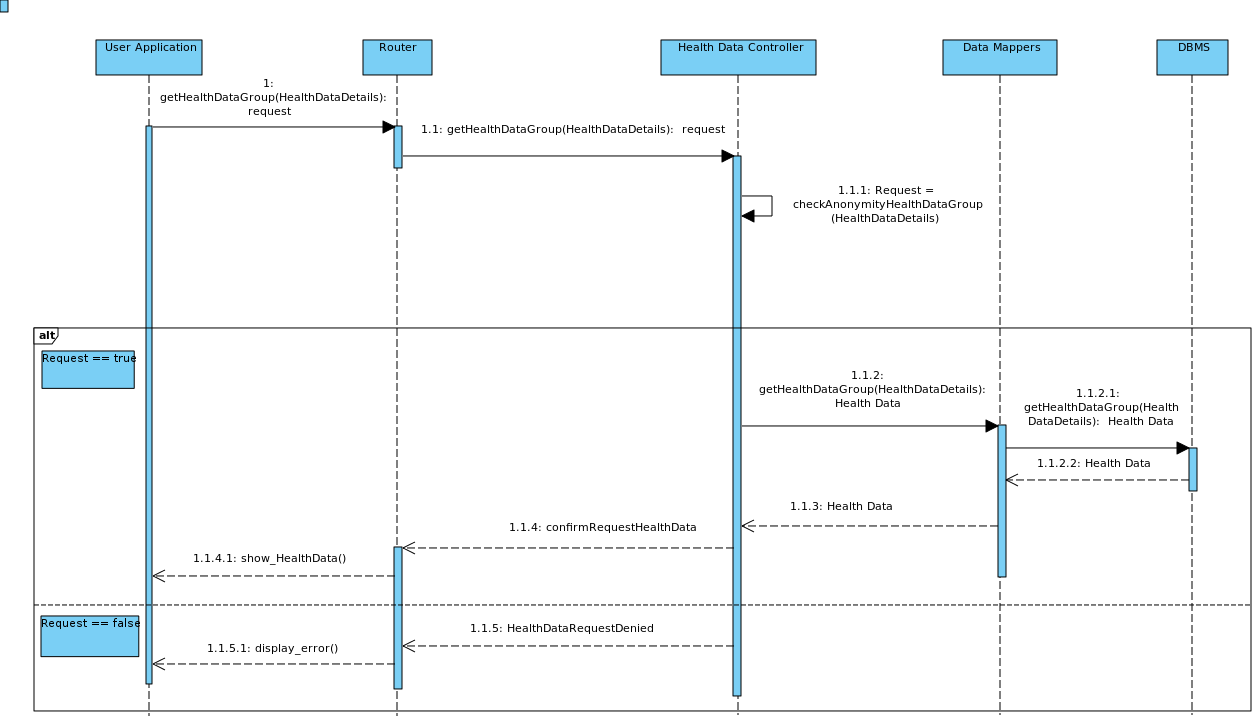
\includegraphics[scale=0.35, angle=-90, origin=c]{getHealthDataGroup.png}
    \caption{Request for the Health Data of an anonymized group of individuals.}
    \label{fig:getHealthDataGroup}
\end{figure}


\subsubsection{Create Run}

\begin{figure}[H]
    \centering
    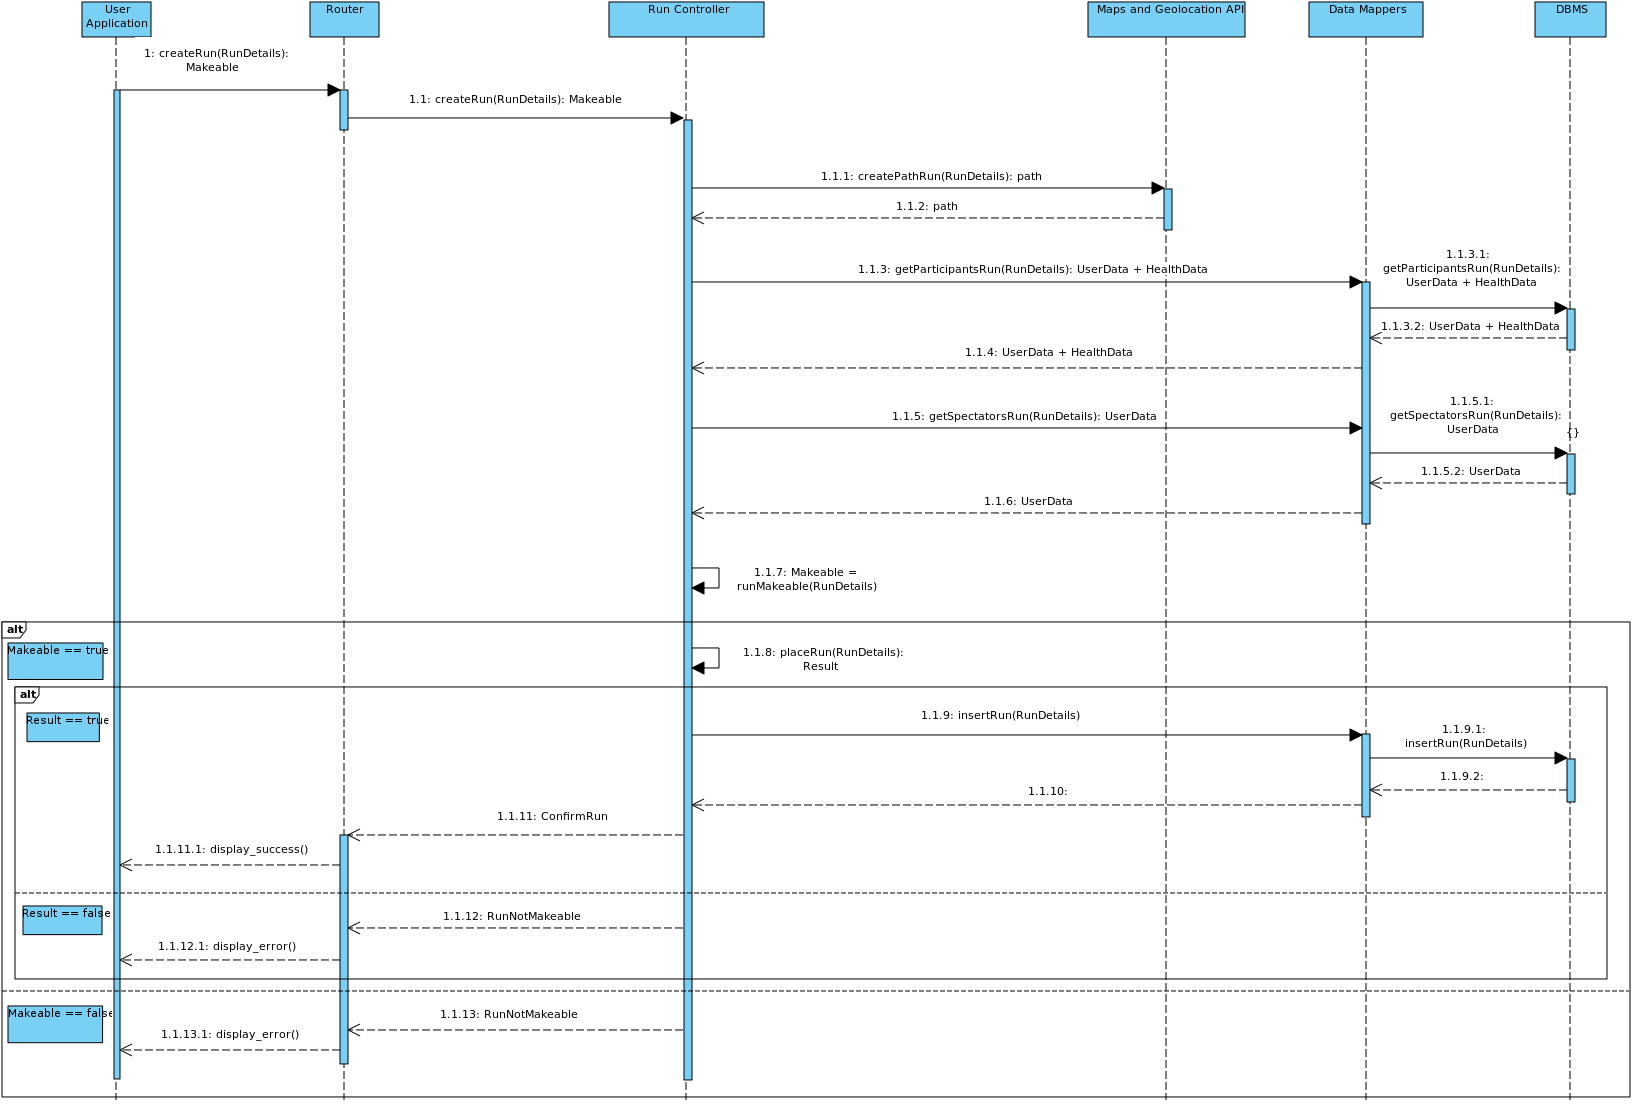
\includegraphics[scale=0.33, angle=-90, origin=c]{createRun.png}
    \caption{Run created by User.}
    \label{fig:createRun}
\end{figure}

\subsection{Component interfaces} 
In this section the interfaces through wich the different system's components interact will be described, and so will will the main methods associated with each interface.

\begin{itemize}
    \item The \textbf{UserAppIntferface} interface represents the way components can interact with the Server, being this the only interface through wich these two can communicate. This interface provides all of the methods provided by the \textbf{HealthDataIntferace} and the \textbf{RunIntferface}
    \item The \textbf{RunIntferface} interface represents the way components can interact with the Run Controller, responsible for managing all of the aspects associated with the run management. This interface provides the following methods: 
    \begin{enumerate}
        \item createRun(string: name, string: description, date: start, location: from, location: to): receives the necessary information to create a run and creates it. 
        \item searchRun(date: start, location: userLocation): receives parameters to search if there are runs organized in the neighboorhood of the given user location. Returns zero or more runId's depending whether a match is found or not.
        \item deleteRun(int: runId): deletes the run with the specified Id. 
        \item enrollRun(int: runId, string: username): adds the user to the list of runners of the specified run.
        \item spectateRun(int: runId, string: username): adds the user and some useful information about them to the list of spectators of a specific run defined by the runId. The user is now capable of spectating/monitoring all the participants of a run.
    \end{enumerate}
    
    \item The \textbf{AccountInterface} represents the way components interact with the Account Controller, responsible for managing all the aspects associated with the user account. This interface provides the following methods: 
    \begin{enumerate}
        \item createAccount(string: username, sting: email, string: password, boolean: individual, boolean: third party): register a visitor into the system, creating an account for him and distinguishing if it is a third party or an individual. 
        \item loginUser(string: username, string: password): logs a user into the system. 
        \item recoverPassword(string: user, string: email) sends a new password to user email, deleting the previous one. 
    \end{enumerate}
    \newpage 
    \item The \textbf{HealthDataInterface} represents the way components interact with the Health Data Controller, responsible for managing the aspects associated with the data accesses policies described previously. This interface provides the following methods: \begin{enumerate}
        \item getData(string: username): import all health data available from a certain user and save them in the system.
        \item requestData(string: username): send a request to a user in order to make its data available for another user. 
        \item acceptRequest(requestId, string: usernameAccept, string: usernameRequest) sends all the data from a user that accepted request to the user that requested them. 
        \item getDataGroup(): sends all the anonimized data of a group of individuals to a user that requested. 
        \item checkData(string: username) priodically checks health data of a certain user in order to monitor if the person is in danger or not.
    \end{enumerate}
    
    \item  The \textbf{DataAccessInterface} represent the way components can interact with the Data Mappers Component. It provides all the needed method and mechanisms to abstract the interaction between database and the system. 
    \item The \textbf{Google Maps and Geolocation API} interface represents the way components can interact with Google Maps and Geolocation service. It provides all the needed methods to get information about the user's location (to attach a location to health data) and for defining a path for run. 
    \item The \textbf{Ambulanza Milano API} interface represents the way components interact with the emergency service of the city of Milan. It provides all the needed methods in order to alert an ambulance when a user is in danger and passes the position of the person in danger to the ambulance service.
    \item The \textbf{HealthKit/Google Fit} interface respresents the way components interact with the health data  service. These two interfaces provide all the needed methods for collecting all possible health data about a user. 
    \item The \textbf{DBMS API} interface represents the way components can interact with the Database. This interface provides the usual methods that are needed to interact with a database, like update, insert, delete and select queries.

\end{itemize}


\subsection{Selected architectural styles and patterns}
\subsubsection{Client/Server Architecture} 
This application is made to run on devices (smartphones and smartwatches) that have limitations regarding memory, storage capacity, computational power and battery. Battery life is usually the most limiting factor in mobile devices. Reading and writing to memory, wireless connections, specialized hardware and processor speed all have an impact on the overall power usage. The application should be optimized to minimize its power and memory footprint while considering performance during this process. So we choose this architectural style in order to keep all the logic of the program, which is computationally quite heavy, on the server side, while the end-users only need to offer a simple amount of presentation and sharing data functionality, avoiding it to use a big amount of memory and CPU. This allows the system to be centralized, which improves: 
\begin{itemize}
    \item Performance: system's files are only accessed by the server, and then sent to the users, so they are always in the same place, becoming easier to manage and faster to acces.
    \item Security: facilitates the implementation of security layers and protocols between the client and the server, setting up access rights to reach server for example. 
    \item Scalability: it is easy to change the logic of the server without any change on the client side.  
\end{itemize}

\subsubsection{Distributed Database} Our system must be able to store big amounts of data belonging to each individual that registers to the application. In order to achieve this we choose to use a distributed database, who will run in different machines. This decision not only gives us an incresead amount of memory, but also gives us the opportunity to make the system more reliable, considering that there is not a single point of failure and a crash of a single machine won't be fatal. Moreover it becomes more scalable because it is easier augmenting the total amount of memory, adding machines to the database. Only one DBMS will be used and the chosen one is mySQL because it is the more used and documentated one. 

\newpage

\subsubsection{Service Oriented Architecture}

This architectural pattern allows the system to be designed as a collection of services that communicate with each other. This way, the external APIs that the system interacts with can be interpreted as a set of these services, which makes them easily implementable (in this case our system is the service consumer, and the APIs are the service providers). It is also possible to see our system as the service provider, first providing an initial set of services and eventually, with the addition of some additional components, increasing the number of services provided.

\subsubsection{Layered Architecture}

The concept of layers is used here in order to maximize separation of concerns between the various components of the system, given that every component operates at a single logical layer of abstraction. Choosing a layered architecture also improves reuse and maintainability for the mobile application. This design choice also simplifies the implementation and testing phase of the system: since the layers are isolated from each other, it is possible to test a specific layer even if the underlying layers aren't implemented, using mocks or stubs to simulate the functionality of those.

\subsubsection{3-Tier Physical Architecture}
The most suitable architecture for the TrackMe application would be three tier architecture. The system will be composed of 3 tiers: Presentation tier, Business tier (the business logic of the system) and Data tier. The Presentation tier is the topmost level of the application. It displays information related to such services as showing all available types of health data, organizing a run, managing your account, etc. It communicates with the other tiers by which it puts out the results to the client. It is the layer which users can access directly (the application's GUI). The Business tier controls the application’s functionality. The Data tier includes the data persistence mechanisms (database servers, file shares, etc.) and the data access layer that encapsulates the persistence mechanisms and exposes the data. The data access layer should provide an API to the Business tier that exposes methods of managing the stored data without exposing or creating dependencies on the data storage mechanisms. Avoiding dependencies on the storage mechanisms allows for updates or changes without the application tier clients being affected by or even aware of the change. This architectural style allows the various components of the system to be deployed on different devices, given the decoupling that exists between the modules. It also allows for any of the three tiers to be upgraded or replaced independently in response to changes in requirements or technology, improving the system’s scalability. As with the separation of any tier, there are costs for implementation and often costs to performance in exchange for improved scalability and maintainability.

\subsubsection{Model-View-Controller}
The TrackMe application core operation is to retrieve health data from our database and update the user 
interface with the newly created data. Therefore we choose a MVC model which divides our
application into 3 interconnected parts, separating the internal representation of information from the 
way this information is presented to the user. This is one of the most used patterns to promote 
decoupling between the major components of a system, allowing for efficient code reuse and parallel 
development. The 3 interconnected parts are: \textbf{Model}, \textbf{View} and \textbf{Controller}. The 
Model is the central component of the pattern. It is the application's dynamic data structure, 
independent of the user interface. It directly manages the data, logic and rules of the application. A 
View can be any output representation of information. We have multiple views e.g.: one view that 
displays all health data available, one view that shows a map where you can track all participants of a 
run. The Controller accepts input and converts it to commands for the model or view. Figure ~\ref{fig:MVC-Process} shows the main interactions between the 3 interconnected parts.
\vspace{10mm}

\begin{figure}[H]
    \centering
    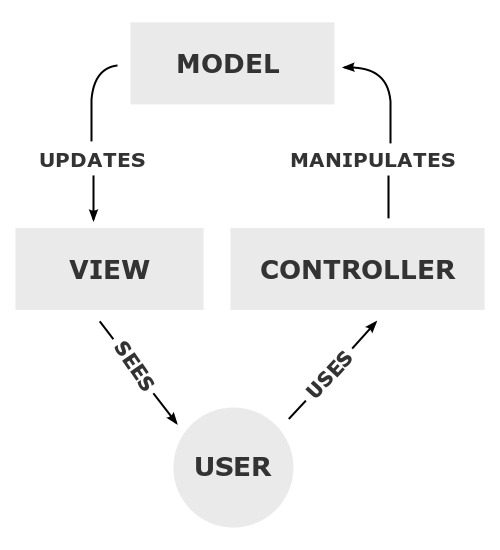
\includegraphics[scale=0.45]{MVC-Process.png}
    \caption{Interactions between the MVC components.}
    \label{fig:MVC-Process}
\end{figure}

\subsubsection{Data Mapper}
A Data Mapper is a Data Access Layer that performs bidirectional transfer of data between our ER 
database and an in-memory data representation (the domain layer). It's responsible 
for transferring data between the two while keeping them isolated from each other and from the mapper
itself. The data mapper consists of a layer of software that separates the in-memory representation and 
the persistent ER database. 

\subsubsection{REST}
A REST architectural style with JSON data model format is also being used to allow the communication 
between the User Application and the Server, this is based on HTTP requests: POST, GET, PUT and 
DELETE are the most important and relevant ones.

\subsubsection{Other design decisions}

\begin{itemize}
    \item \textbf{Application Server}: GlassFish 5.0 was chosen since it provides containers
          for both the EJB and the JSP pages, and is a full JEE Application server.
\end{itemize}



 
\section{Algorithm design}
In this section an overall descripition is presented of the most relevant algorithms used for the TrackMe 
application, explained using pseudocode notation. 
\subsection{Track4Run service algorithms}

\subsubsection{Run Placement Algorithm}
This algoritm controls if it's possible to create a run in a certain moment and location, checking if there
are some other runs that prevent to do it. 
When a user tries to create a run there are 4 possible situation:
\begin{itemize}
    \item There is not any other run at that time or location. 
    \item There is another run at the same time but the location is different. 
    \item There is another run in the same location but it has a different timetable. 
    \item There is another run at the same time and same place 
\end{itemize}

\begin{algorithm}[H]
\textbf{Run1:(Start1,End1,Track1)} run to be inserted must have a start time, an end time and a track\; 
$F\leftarrow 0$   - no overlapping runs\;
\noindent \ForEach {Run:(Start,End;Track) in the set of runs}{
\eIf{Start1$>$End $\lor$ End1$<$Start $\lor$ Track1 $\cap$ Track = $\emptyset$} {Run can be created} 
{$F\leftarrow 1$\; \vspace{1mm}
 Run cannot be created\; \vspace{1mm}
 Exit from the algorithm\; \vspace{1mm}
 }

}

\end{algorithm} 


\subsubsection{Run enrollment algorithm}  

The pourpose of its algorithm is to control the enrollment of a run by an individual. The alghoritm checks if there are some overlapping runs and the health status of the individual, in order to avoid that a unhealty person can join a run. 

\begin{algorithm} 
\textbf{Run1(Start1,End1,Track1) and Individual Health Status} \;
$F \leftarrow 0;$ \;
\While{ F $\neq$ 1 }{ 
\eIf{Indiviadual Health Status $\neq$ Healty}
{$F \leftarrow 1$ \; 
Race cannot be enrolled } {Race can be enrolled}
\noindent \ForEach{Run(Start,End;Track1) in runs enrolled by the individual}
{\eIf {Start1 $>$ End $\lor$ End1 $<$ Start} { Run can be enrolled}{F$\leftarrow$1 \; Race cannot be enrolled}

}
}


\end{algorithm}

\subsection{Data4Help service algorithms}

\subsubsection{Health Data Acquisition by Individual Algorithm}

This algorithm controls the acquisition of all available health data of an individual that is generated by 
smartphones, smartwatches or other external devices. This algorithm is performed by the system in the 
background as the individual doesn't need to click on a button to retrieve his health data.
\vspace{10mm}

\begin{algorithm}[H]
 \textbf{Individual:} the current username of the individual who uses the TrackMe\;
 \noindent \textbf{Devices:} get a list of the external devices that the Individual uses\;
 \noindent \For {every Device in Devices}{   
    read ervery tuple (data, dataType) from Device\;  \vspace{1mm}
    add the current Location of the Individual to each (data,dataType)\;   \vspace{1mm}
    pushed = try to push the tuples (data, dataType, Location) to DB\;   \vspace{1mm}
    \eIf{pushed == True}{     
    continue\;    
    }
    {    
    go back to try push the tuples to the DB\;   
    }  
    }
 \noindent \For {every dataType in DB}{   
    read every tuple (data, dataType, Location)\;  
    }
    update the user's screen by showing the latest health data per dataType\;\vspace{1mm}
    repeat the process starting from the first for loop every x seconds;
 \vspace{5mm}
 \caption{Health Data Acquisition by Individual.}
\end{algorithm}

\newpage
\subsubsection{Access Health Data of an Individual Algorithm}

This algorithm controls the request of an third party to access all available health data of an 
specific individual.
\vspace{10mm}

\begin{algorithm}[H]
 \textbf{Fiscal Code:} the fiscal code of the individual\;
 \vspace{1mm}
 the third party sends a request to the system using the fiscal code\;\vspace{1mm}
 the system forwards this request to the individual belonging to the fiscal code\;\vspace{1mm}
 request = get the response of the individual to monitor his health\; \vspace{1mm}
 \eIf{request == True}{
    inform the third party that the request is approved\; \vspace{1mm}
    read the previously saved health data belonging to the fiscal code from the DB and show it to the third party\; \vspace{1mm}
    listen for the latest health data and update the third party's screen as soon as new data is produced\;    
    }
    {    
    inform the third party that the request is denied\;   
    }  

    
 \vspace{5mm}
 \caption{Access Health Data of an Individual.}
\end{algorithm}


\newpage
\subsubsection{Access anonymized Health Data of groups of an Individuals Algorithm}

This algorithm controls the request of an third party to access anonymized data of groups of individuals.
\vspace{10mm}

\begin{algorithm}[H]
 \textbf{Search variable:} the variable the third party provides to search for groups of individuals that satisfy the variable\;
 \vspace{1mm}
 the third party sends a request to the system providing the search variable\;\vspace{1mm}
 request = the system internally handles this request and checks how many individuals are found\;\vspace{1mm}
 \eIf{individuals $>$ 1000 in request}{
    anonymized == True \;    
    }
    {    
    anonymized == False\;   
    }  
 
 \eIf{anonymized == True}{
    inform the third party that the request is approved\; \vspace{1mm}
    read the previously saved health data belonging to groups of individuals from the DB and show it to the third party\; \vspace{1mm}
    listen for the latest health data and update the third party's screen as soon as new data is produced\;
    }
    {    
    inform the third party that the request is denied\;   
    }  
 \vspace{5mm}
 \caption{Access anonymized Health Data of groups of an Individuals.}
\end{algorithm}

\newpage

\subsection{AutomatedSOS service Algorithm}
This algorithm monitors the health data of every individual who uses the TrackMe application. If a certain  parameter of an individual drops below a value the system pushes a request to the Ambulanza Milano to send an ambulance to the individual in danger.
This algorithm below is applied to every individual in the system.
\vspace{5mm}

\begin{algorithm}[H]
 \textbf{Health Data:} health data (values) for an individual using the TrackMe service\;
 \vspace{1mm}
  \textbf{Threshold:} a list of thresholds for every type of health data\;
 \vspace{1mm}
 parameters = dictionary with structure (keys:health data,values:threshold)\;\vspace{1mm}
 \noindent \For{every parameter in parameters}{
 \eIf{parameter $<$ Threshold}{
    health status = in danger\;
    guarantee reaction time less than 5 seconds to send ambulance to individual in danger\;
    arrival of ambulance\;
    health status = healthy\;
    }
    {    
    continue\;   
    }}  
 repeat the algorithm every x seconds;
 
 \vspace{5mm}
 \caption{AutomatedSOS service.}
\end{algorithm}

\newpage
\section{User Interface design}

\subsection{Mockups} One of the most important things when designing a information system is the way its functionality is presented and provided to the user. It is imoprtant to guarantee semplicity and the system should be easy to use for everyone, expecially in the case of an application devoted to a big ammount of users. For that reason the user interface should be as simple and intuitive as possible, in order to let the user know what it is doing easily. 
    Another important aspect that is important to take into consideration is the adaptibility of our software for every type of smartphone. For that reason the user interface is very minimalist, without details and animation that could made the application impossible to run in certain types of smartphones. The mockups of the UI can be found in the RASD document under \textbf{section 3.1.1}.
    
\subsection{UX diagram} 

The following UX Diagram provides addictional information about the way the user interacts with the system through the mobile application, with the pourpose of complementing the UI mockups provided in the RASD document. 

\begin{figure}[H]
    \centering
    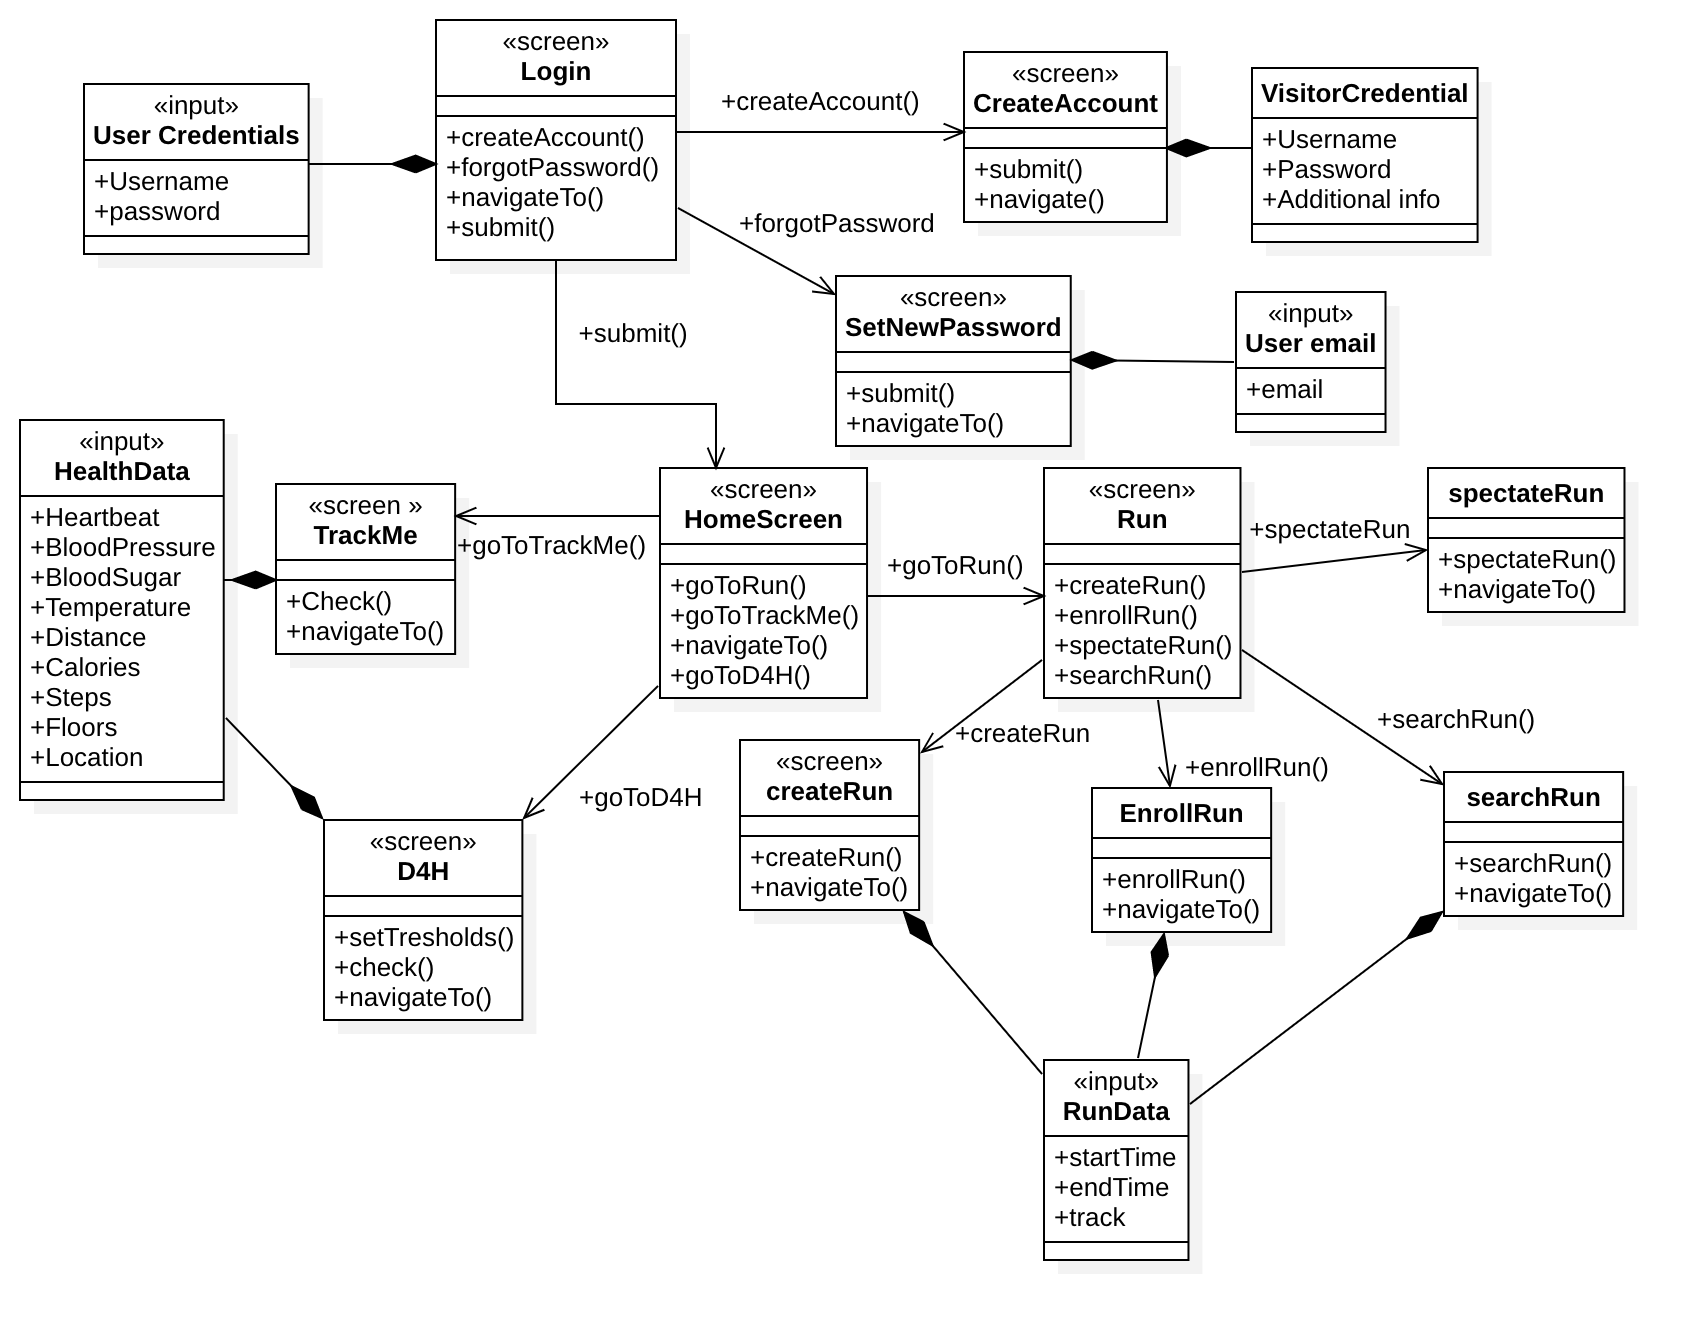
\includegraphics[scale=0.33, angle=-90, origin=c]{UXdiagram.png}
    \caption{UX diagram.}
    \label{fig:UX diagram}
\end{figure}


\section{Requirements traceability}
\subsection{Functional Requirements}
All of the design choices presented in this document were made with the goals and requirements defined in the RASD in mind and aim to fulfill them in the best possible way. The following list provides an accurate mapping between the system's goals and requirements defined in the RASD and the system components, defined in the DD, that aim to fulfill those goals and requirements.
\newline \textbf{N.B.: All the requirement intervals include the first and the last on the interval.}

\begin{itemize}
    \item \textbf{[G1]} Allow a visitor to become a registered individual or third party after providing email, username/organization, password, general info (if case of an individual) (R1-R4). 
\begin{itemize}
    \item The \textbf{Account Controller} provides the visitors the ability to register as an individual or third party of the system.
\end{itemize}

\item \textbf{[G2]} Allow a user to monitor it’s health status. (R5-R7) 
\begin{itemize} 
    \item The \textbf{Health Data Controller} provides an individual all of the business logic related to monitor it's health data. The system receives data from external devices, stores it in the system's database and shows it on the individual application screen.
\end{itemize}

\item \textbf{[G3]} Allow third parties to request data from a specific individual after authorization. (R8-R11)
\begin{itemize}
    \item First the \textbf{Account Controller} communicates with a specific individual to ask for the permission to acces his health data. After permission, the \textbf{Health Data Controller} provides the third party off all the business logic related to monitor the individual's health data.
\end{itemize}
\item \textbf{[G4]} Allow third parties to subscribe to new data and receive them as soon as they are produced. 
\begin{itemize}
    \item The \textbf{Data Access Controller} provides a third party the ability to access new data as soon as they are produced.
\end{itemize}
\newpage
\item \textbf{[G5]} Allow third parties to access anonymized data of a group of individuals. (R12-R13)
   \begin{itemize}
       \item The \textbf{Data Access Controller} provides a third party the acces to anonymized data after the \textbf{Health Data Controller} approved that it is able to properly anonymize the requested data.
   \end{itemize}  
 \item \textbf{[G6]} Allow individuals to choose what data is being send to the application’s DB. (R14-R16)
   \begin{itemize}
       \item The \textbf{Account Controller} manages the health data preferences from an individual so it can control which health data is send to the DB.
    \end{itemize}
 \item \textbf{[G7]} Allow third parties to acquire data from Data4Help. (R17)
       \begin{itemize}
           \item The \textbf{Data Access Controller} provides third parties to access data about individuals.
       \end{itemize}
  \item \textbf{[G8]} Allow individuals to define a certain threshold for a certain parameter. (R18-R19)
        \begin{itemize}
            \item The \textbf{Account Controller} provides individuals a way to define a certain threshold for a parameter.
        \end{itemize}
  \item \textbf{[G9]} Call an ambulance when parameters drop below a certain threshold. (R20-R22)
        \begin{itemize}
            \item The \textbf{Health Data Controller} communicates with the Ambulanza Milano API to request an ambulance in case an individual is in danger.
        \end{itemize}
  \item \textbf{[G10]} Allow an individual/third party to organize a track for a run. (R23-R25)
        \begin{itemize}
            \item The \textbf{Run Controller} provides an individual/third party to organize a run by choosing a path.
        \end{itemize}
  \item \textbf{[G11]} Allow an individual/third party to enroll for a run. (R26-R27)
        \begin{itemize}
            \item The \textbf{Run Controller} provides an individual/third party the ability to enroll for a certain run.
        \end{itemize}
  \item \textbf{[G12]} Allow an individual/third party to see the live position of all runners during the run. (R28)
        \begin{itemize}
            \item The \textbf{Run Controller} in combination with the \textbf{Health Data Controller} provides the ability to monitor the activities of participants runnners and show their realtime positions on the map.
        \end{itemize}
        
        
\end{itemize}

\subsection{Non-Functional Requirements}

The non-functional requirements were no exception and were also taken into consideration when making the Design Choices for the system. In particular, this analysis will be focused on the \textbf{Performance, Reliability, Availability, Security}, and \textbf{Portability} requirements.

\noindent The usage of a 3 tier infrastructure is the key to achieve most of these requirements. This infrastructure allows us not only to achieve high levels of \textbf{Performance} (components with different hardware needs can be deployed in more powerful machines) but also satisfying levels of \textbf{Reliability} and \textbf{Availability} as, thanks to the low coupling between the different components, it allows them to be distributed over the network, possibly replicated and in different server farms (highly increasing fault tolerance).

\noindent \textbf{Security} is achieved thanks to software and hardware steps. At the software level, all interface methods check if the call parameters are valid before executing its main logic and if the caller is authorized to invoke them. The database APIs will also be protected against SQL Injection and all messages between different components of the system and external APIs will be encrypted and will have unique identifiers. Using this level of encryption we proctect all the critical data and prevent man-in-the-middle attacks (more specifically replay attacks).

\noindent At last, \textbf{Portability} is achieved by offering a standard web service mechanism based on JSON through the API's. This allows the system to be invoked from any platform with internet access, not restricting the system to a specific operating system, programming language or hardware brand.

\section{Implementation, Integration and Test Plan}
Implementation, Integration, and Testing are 3 differenterent activities that must be done
together in order for a project to be developed in a correct way. In the paragraphs below we will present a
plan for the implementation, integration, and testing of the different components that, together, form our 
system.
The system is divided into layers, and as in a traditional layered architecture,
the topmost layers depend on the lowest ones. This being said, the system must be
implemented using 1 out of 3 differentrent approaches:
\begin{itemize}
    \item Bottom-Up approach
    \item Top-down approach
    \item Mix between Bottom-Up and Top-down, which meet somewhere in the middle 
     
\end{itemize}

\noindent The second and third approaches imply that a component will be implemented
and tested without the need for the components that this depends on to be implemented and tested already. 
Although this might look like a good idea, it carries a
more complex development process, since mocks would have to be built in order to
test the behavior of these components after being implemented. Taking this into
consideration, the approach chosen to develop our system was a bottom-up
approach. This way, the components which do not depend on others will be the
first ones to be developed and extensively tested, followed by the ones that only depend on those, until we reach the highest layer of the system, with the components
that have no other component depending on them. Thanks to this a component can
be tested and integrated as soon as it's finished (or even close to being finished),
allowing us to complete the development and testing phase almost in parallel. We
must also keep in mind that in order to test the integration of two components, the
main features of both of them should have already been developed and the related
unit tests should have been performed.
\subsection{DBMS}
The first component to be implemented is the DBMS. It shall be implemented and then fully tested before finishing the implementation of the layer above since it has
to be configured and operative in order to allow to test all of the components which need access to the database.
\subsection{Server}
The next set of components to be implemented and tested are the ones that belong to the Business Layer, which encapsulates the business logic of the system. This layer is composed of the Server component and all of its sub-components.
\newline \noindent First, we should start with the \textbf{Data Mappers} sub-component, which is the Server component that mediates the interaction between the server and the database, and only depends on the DBMS component.
\newline \noindent After this, and following a critical-module-first approach, we should develop the \textbf{Health Data Controller}, \textbf{Run Controller} and the \textbf{Data Access Controller} components, in particular the \textbf{Health Data} component. Both the \textbf{Health Data Controller} and \textbf{Run Controller} require the interaction with the external services to be fully functional. The last sub-components of the server to be developed will be the \textbf{Account Controller} and \textbf{Router Controller}. 
\newline \noindent After being fully implemented, the Server component must be integrated with
the DBMS component, as it needs the DBMS to work properly.
\newline \noindent Before integration testing of the two integrated components, the used external
services shall be configured and fully operative. After this, the Server can be integrated with the DBMS and shall be extensively tested, as it is the most critical and important part of the system. 
\subsection{User Applicaton}The final part of the system to be implemented is the User Application, the topmost
layer of the architecture. Since we opted for a thin client this shall be one of the
easiest and fastest steps of the development process. When finished, it shall be
integrated with the rest of the components of the system in order to test the system
as a whole.





\section{Effort spent}

\subsection{Michiel Janssen}

\begin{center}
\begin{tabular}{ |p{0.25\textwidth}|p{0.4\textwidth}|p{0.25\textwidth}| } 
 \hline
 \textbf{DATE} & \textbf{TASK} & \textbf{HOURS} \\ 
 \hline 
  28/11/2018 & Purpose, Scope, Definitions, Acronyms, Abbreviations & 2,5\\
  \hline
  29/11/2018 & High-level Components Description, Component View & 6\\
  \hline
  30/11/2018 & Database detailed analysis, Deployment View, Runtime View & 6,5\\
  \hline
  01/12/2018 & Server detailed analysis, Deployment View, Runtime View, Component Interfaces & 4,5\\
  \hline
  02/12/2018 & Runtime View, Architectural style & 3,5\\
  \hline
  03/12/2018 & Architectural style, Requirements traceability & 3\\
  \hline
  04/12/2018 & Implementation, Integration and Test Plan, Algorithm Design & 4 \\
  \hline
  05/12/2018 & Algorithm Design & 2\\
  \hline
  \textbf{TOTAL} & \multicolumn{2}{c|}{32} \\ 
  \hline
\end{tabular}
\end{center}


\subsection{Erbol Kasenov}

\begin{center}
\begin{tabular}{ |p{0.25\textwidth}|p{0.4\textwidth}|p{0.25\textwidth}| } 
 \hline
 \textbf{DATE} & \textbf{TASK} & \textbf{HOURS} \\ 
  \hline
  18/11/2018 & Timetable, Purpose, Scope, Definitions, Acronyms, 
  Abbreviations, References document, Document Structure & 4,5\\ 
  \hline
  01/12/2018 & Implementation, Integration and Test Plan & 1,5\\ 
   \hline
  03/12/2018 & Requirements traceability & 2 \\ 
  \hline
  08/12/2018 & Definitions, Acronyms & 1\\
  \hline
  \textbf{TOTAL} & \multicolumn{2}{c|}{9} \\ 
  \hline
\end{tabular}
\end{center}

\subsection{Lorenzo Casalini}

\begin{center}
\begin{tabular}{ |p{0.25\textwidth}|p{0.4\textwidth}|p{0.25\textwidth}| } 
 \hline
 \textbf{DATE} & \textbf{TASK} & \textbf{HOURS} \\ 
  \hline
 01/12/2018 & Component Interfaces, Architectural style & 4\\
 \hline 
 02/12/2018 & Algorithm Design & 2 \\
 \hline
 03/12/2018 & User Interface Design & 3,5\\ 
 \hline 
 05/12/2018 & Algorithm Design & 4\\
  
  \hline
  \textbf{TOTAL} & \multicolumn{2}{c|}{13,5} \\ 
  \hline
\end{tabular}
\end{center}







\end{document}